% Therapeutischer Prozess
% ***********************
\section{Therapeutischer Prozess}\label{Prozess}
In diesem Kapitel werde ich auf den eigentlichen therapeutischen Prozess eingehen. Darin enthalten sind die Auftragsklärung, die Beziehungsgestaltung, die Diagnostik nach ICD Richtlinien, die Hypothesenbildung und Interventionen, sowie der Verlauf.   

Da es sich beim Fall SK um einen länger andauernden Fall handelt, der zudem noch nicht abgeschlossen ist, möchte ich in einem ersten Schritt die bisherigen Stationen anhand eines Zeitstrahls abbilden (siehe \textit{Abbildung\ref{fig:Behanldungsepisode}: \titleref{fig:Behanldungsepisode}}). Dadurch soll die Orientierung im Text verständlicher werden. Zudem ermöglich mir diese grafische Abbildung weiter unten im Kapitel \titleref{Verlauf} auf einzelne Abschnitte, sowie Ereignisse genauer eingehen zu können. Diese Orientierung soll auch im nächsten Kapitel \titleref{sec:TherapeutischeWechselwirkung} Verwendung finden. 

\begin{figure} 
    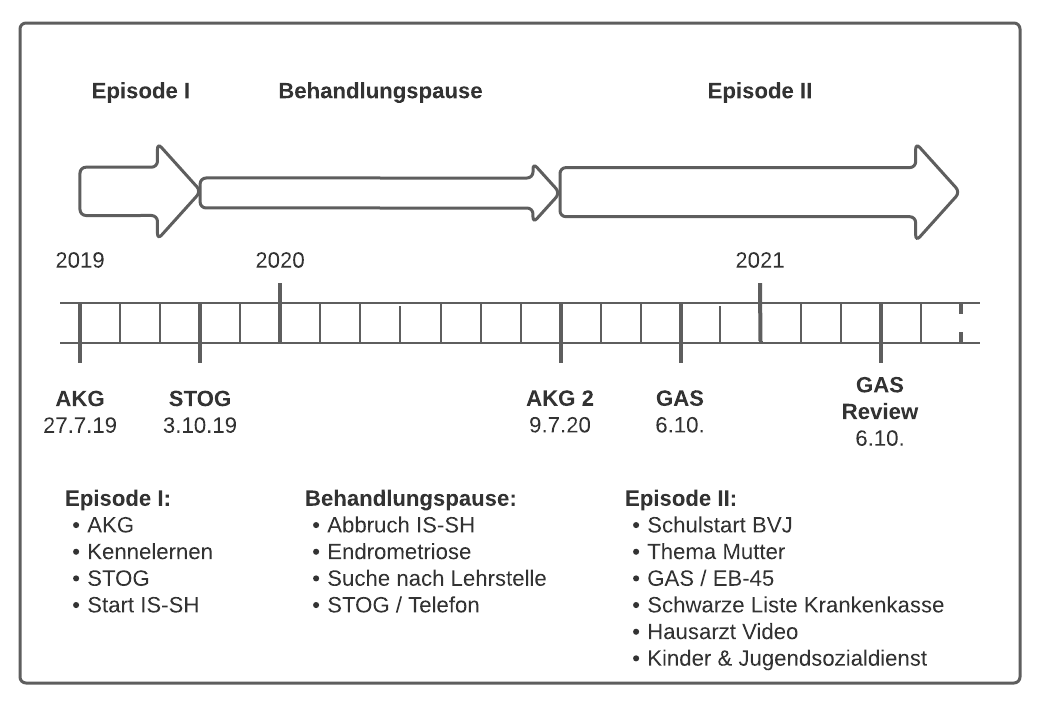
\includegraphics[width=0.95\textwidth]{pictures/Zeitstrahl_Fall_SK.png}
    %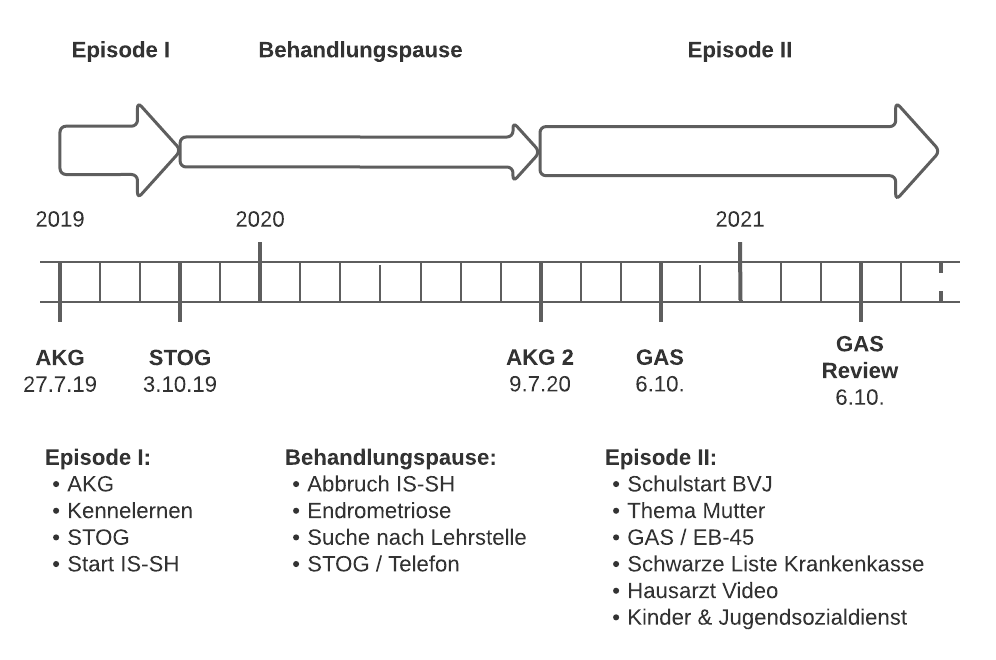
\includegraphics[width=0.95\textwidth]{pictures/Zeitstrahl_Fall_SK_ohneRahmen.png}
    \caption{Behandlungsepisoden}
    \label{fig:Behanldungsepisode}
\end{figure}

\subsection{Auftragsklärung}\label{Auftragsklärung} 
Gemäss \citeA{Wampold2015} gehört die Übereinstimmung der Ziele von Therapeut*in und Klient*in zu den allgemeinen Wirkfaktoren. Beim ersten \acf{akg} mit SK und ihrer Mutter verfolgte ich intuitiv diesen Ansatz. Wie ich mir aus dem Psychologiestudium in der Vorlesungen humanistischen Therapie gemerkt habe ist es wichtig, die Anliegen und Wünsche der Klienten zu verstehen (mit der systemischen Ausbildung am IEF habe ich erst kurz nach dem ersten Gespräch begonnen). 

Für das erste \ac{akg} hielt ich mich an die am \ac{kjpd} übliche Vorgehensweise: Dazu gehört in die Einleitung die \textit{Festlegung des Gesprächsziels}, welches dazu führen soll zu entscheiden, ob der \ac{kjpd} die richtige Stelle für das Anliegen der Klienten ist und bei dem es darum geht mit den Klienten ein gemeinsames Verständnis für das Anliegen zu erarbeiten. Weiter gehört eine kurze \textit{Vorstellung der Institution}, sowie die Schilderung des \textit{Ablaufs} dazu, bei dem ich auf den zeitlichen Rahmen, die Institution und das grobe Vorgehen im Gespräch eingegangen bin. Bei der Schilderung von \textit{Anmeldegrund \& Problembeschreibung} wurde bereits klar, dass die Mutter die Anmeldung aus eigenem Wunsch vorgenommen hatte. Dabei sei es in der Vergangenheit zu Konflikten zwischen der Schule und SK gekommen, da diese krankheitsbedingt viele Fehltage hatte und die Schule dies nicht mehr länger akzeptieren wollte. Für die Problembeschreibung holte die Mutter weit aus und schilderte aus ihrer Sicht die Entstehung des Anliegens. SK war während der gesamten Ausführung der Mutter erstaunlich ruhig. Sie meldete sich dabei nicht aktiv zu Wort und korrigierte die Mutter auch nicht. Ich stellte die Vermutung an, dass primär die Mutter ein Anliegen für die Anmeldung hatte, SK die Verantwortung ihrer Mutter übergab und selber kein direktes Anliegen vorzuweisen hatte. Beim Abschnitt \textit{Reaktionen auf das Problemverhalten} ergaben sich Hinweise auf Mobbingsituationen an der Schule und einer vor ein paar Jahren stattgefundenen Trennung der Eltern, auf die SK mit Schulangst und Rückzugstendenzen reagierte. Leider konnte ich bei diesem Gespräch weder von SK noch von ihrer Mutter Hinweise auf \textit{Erklärungsansätze} in Erfahrung bringen. Ich ging implizit davon aus, dass SK und die Mutter das Verhalten von SK mit der Mobbingerfahrung und der schwierigen Schulsituation in Verbindung brachten. Hier hätte ich aus aktueller Sicht das Bedürfnis, die Anwesenden nach ihren eigenen Erklärungsansätze zu fragen. Bei den \textit{Bisherigen Massnahmen, resp. Lösungsversuche} wurde von der Mutter berichtet, dass SK nach einem erfolglosen Schulwechsel in eine Privatschule aufgrund der Mobbingsituation für ein paar Monate stationär in einer Klinik behandelt wurde. In diesem Zusammenhang sei die Diagnose Depression und eine zugehörige Angsterkrankung diagnostiziert worden. Im Anschluss an den Klinikaufenthalt wurde eine ambulante Nachbetreuung installiert, in Form einer Therapeutin und einer  psychiatrischen Spitex. Die Mutter berichtete weiter, dass sich das Verhältnis zwischen SK und dem behandelnden Psychiater verschlechterte und die Mutter das Therapiebündnis beendete. Daraus entstand das explizite \textit{Anliegen} an mich, die ambulante Betreuung von SK zu übernehmen. Während dem Gespräch hatte ich zudem die Hypothese, dass es sich mindestens um einen weiteren Auftrag handeln würde. Nämlich der, dass ich in Form eines Bündnisses mit der Mutter die Fehltage von SK gegenüber der Schule vertreten sollte. Als ich die Mutter darauf angesprochen habe, bestätigte sie mir dies. Die Mutter wollte der Schule aufzeigen, dass die Absenzen von SK begründet waren und sie als Mutter gut für SK sorgen könne. SK selber wollte an ihrem Selbstvertrauen arbeiten, da sie dort ihre Schwierigkeiten sah. Als ich sie direkt auf die Diagnosen aus der Klinik angesprochen habe, lehnte SK eine Unterstützung diesbezüglich ab, da sie selber damit klar komme. Ich akzeptierte dies, gab jedoch zu bedenken, dass mir der Auftrag für eine Therapieübernahme vorerst noch nicht so ganz klar sei, weshalb ich zu weiteren Terminen in Form von Einzeltermine mit SK riet, um die Auftragsklärung abzuschliessen und im Anschluss das weitere Vorgehen gemeinsam zu besprechen. Auf diese Empfehlung konnte sich die Mutter und SK einlassen.

Nach einer längeren Therapiepause, welche in etwa ein halbes Jahr dauerte, schilderten mir SK und ihre Mutter bei einem Standortgespräch, dass sich SK für das 10. Schuljahr entschieden habe. SK konnte kein Anliegen mehr an mich richten und aufgrund der sich wechselnden Schulsituation hatte sich auch das Anliegen der Mutter erledigt, weshalb die beiden den Fall gerne abschliessen wollten. Zwei Monate später meldete sich SK jedoch selbständig am \ac{kjpd}. Dabei stellte sich heraus, dass SK ein neues Anliegen an mich hatte. Wir führten ein weiteres Auftragsklärungsgespräch durch, welches ich in Absprache mit der Mutter mit SK alleine führte (SK wurde kurz darauf volljährig). Da ich den Fall noch nicht abgeschlossen hatte, entschied ich mich in Rücksprache mit meinem Vorgesetzten den noch laufenden Fall zu verwenden und weiterzuführen. Zum Zeitpunkt des zweiten \acp{akg} befand ich mich bereits am Ende des ersten Jahres meiner Weiterbildung am \ac{ief}, weshalb ich meinen Fokus verstärkt auf die Passung der Ziele legte. Bereits in diesem zweiten Gespräch schilderte mir SK von ihrer aktuellen depressiven Verstimmtheit und den Schlafschwierigkeiten. Zudem hätte sie eine somatische Diagnose erhalten, welche sie sehr belasten würde und über die sie gerne mit mir sprechen würde. Sie habe in der ersten Phase der Therapie bei mir von den Gesprächen profitieren können und erhoffe sich eine Wiederholung der emotionalen Erleichterung. Zudem wollte SK über ihre Schlafschwierigkeiten sprechen, um einen Umgang damit zu finden. In diesem Gespräch wollte ich den Grund der Wiederanmeldung prüfen und die expliziten Ziele grob umreissen. Dabei war es mir wichtig, dass SK aus eigener Motivation eine Therapie anstrebte und nicht von der Mutter geschickt wurde. Nach dem ersten klärenden Gespräch entschieden wir uns für weitere Gespräche, um die Therapieziele gemeinsam zu erarbeiten. Diese Zielerarbeitung erfolgte in den kommenden Sitzungen anhand einer detaillierten Zieldefinition mittels \ac{gas}, auf welche ich im Kapitel \titleref{sec:Evaluationsverfahren} näher eingehen werde.

Die beiden \acp{akg} unterschieden sich nicht nur hinsichtlich meiner eigenen Erfahrung bezogen auf meine Weiterbildung und Therapieerfahrung, sondern auch hinsichtlich der Motivation von SK. War mir die Motivation von SK für eine Therapie in der ersten Behandlungsphase nicht so ganz klar, so wurde diese durch die nun vorgebrachten Anliegen von SK spürbar. Standen beim ersten Gespräch die Anliegen der Mutter im Zentrum, so kamen beim Gespräch mit SK ihre eigenen Bedürfnisse zum Vorschein und leiteten die zweite Behandlungsphase ein. 

%TODO: Überarbeitung

\subsection{Beziehungsgestaltung} \label{lbBeziehungsgestaltung}  
In diesem Kapitel werde ich auf die \titleref{lbBeziehungsgestaltung} in Form des Drei-Kreis-Modells der therapeutischen Beziehung gemäss \citeA{Borst2018} eingehen. Im äussersten Kreis des organisatorischen Rahmens handelt es sich beim \ac{kjpd} um eine öffentliche ambulante psychiatrische Institution, die ärztlich geführt wird. Das heisst aus meiner Sicht, dass grundsätzliche historisch bedingt eine störungsorientierte Sichtweise vorliegt, mit allem was dazu gehört und natürlich auch den klinischen Diagnosen nach ICD-10. Meine Rolle als Psychologe, welches sich zu Beginn an einem humanistischen Bild orientierte und mit Beginn meiner Ausbildung mit einem autonomieorientierten, sowie heteronomieorientierten Menschenbild ergänzte, wirkte dem tendenziell defizitär vorherrschenden Menschenbild entgegen. Während meinem Studium veränderte sich auch mein therapeutische Grundhalten, um eine in Richtung spezifisch-systemischer weisender Grundhaltung. Dadurch, dass ich zu Beginn der Behandlung primär versuchte durch Neugier die Klientin und deren Anliegen zu verstehen, verfolgte ich mit der Zeit eine nicht-invasive und freundliche therapeutische Grundtugend zu etablieren \cite{Cecchin1988}. Dies erfolgte jedoch intuitiv und ermöglichte mir ein erstes Vertrauen von SK zu gewinnen. Im Verlauf der Therapie ergänzte ich meine Grundhaltung, indem ich hypothesengeleitete Fragen zu stellen begann \cite{Andersen1990}, die für SK interessant und angemessen, jedoch ungewöhnlich waren. Dadurch verfolgte ich das Ziel, SK auf neue Gedanken zu bringen und ihr ein vertieftes Verständnis über sich zu ermöglichen. Weiter folgte die Zirkularität, welche den Fokus der Problembeschreibung von SK als Interaktion in der Familie und im grösseren System einordnete und weg von einer individuellen Störung führte. Etwas distanziert betrachtet würde ich behaupten, dass mir dieses Vorgehen ermöglichte mit SK an den Punkt vorzustossen, an dem wir nun sind. Anfänglich konnte SK kein wirklich eigenes Anliegen benennen und es hatte den Anschein, als wollte sie ihre Mutter ruhig stellen. Mit der Zeit jedoch konnte SK genau diese Interaktion innerhalb der Familie und der Mutter als ein sie störendes Element identifizieren, was wiederum zu einer Vertiefung und Festigung der Beziehung aufgrund von diesem Erfolg zwischen SK und mir führte.

Bezogen auf den interaktionellen Rahmen ist in diesem Fall zu bemerken, dass sich auch dieser fortlaufend veränderte und anpasste. Mutete das Anliegen der Mutter an mich zu Beginn nach Kontrolle über SK an, veränderte sich dies zunehmend in Richtung Hilfe zur Selbsthilfe für SK. Das Anliegen der Mutter, einerseits die Schule ruhig zu stellen, indem sie SK beim \ac{kjpd} anmeldete, und andererseits implizit SK hilflos zu halten, indem das Problem bei SK verortet wurde, trat dieses Anliegen zunehmen in den Hintergrund und liess Platz für das eigentliche Anliegen von SK. Dies erfolgte mit einer Abnahme des Einbezugs der Mutter aufgrund der Volljährigkeit von SK. Dies ermöglichte zudem eine gewisse Übernahme von Verantwortung auf der Seite von SK, da sie nun selber für sich entscheiden musste, welche Themen sie bei mir behandeln wollte. Zudem meldete sich der Hausarzt von SK mit einem direkten Anliegen an mich, welches ich zuerst mit SK klären und besprechen musste. Diese von mir angesteuerte Transparenz führte wohl zusätzlich dazu, dass mit SK immer wieder das Vertrauen aussprach und weiter regelmässig in die Therapie kam. 

Innerhalb des innersten Bestimmungsstück der Beziehung zwischen SK und mir, in der affektlogischen Rahmung, verfolgte ich die Metastabilisierung eines instabilen Systems, ohne jedoch die Grundstruktur des Systems zu verändern. Bisher ist mir dies gelungen, jedoch gab es Episoden, an denen die Grundstruktur bei SK gefährdet wurde, indem sie sich für das Verlassen des familiären Systems ausgesprochen hatte. Aus meiner Sicht hätte dieser Schritt zu einer Systemveränderung geführt, welcher im Extremen mit dem Bruch der Familie, insbesondere der Beziehung zur Mutter, geführt hätte. Diesbezüglich fand jedoch eine erneute Beruhigung statt, auf der weiter aufgebaut werden konnte. 

Es war mir nicht möglich diese drei Kreise gesondert zu betrachten, da sich diese  gegenseitig beeinflussen. Dadurch, dass ich SK bereits über mehrere Jahre begleite, veränderte sich einerseits bei Sarina die Aufträge dritter im organisatorischen Rahmen (obligatorische Schule, 10. Schuljahr, Mutter), sowie das Anliegen von Dritten im interaktionellen Rahmen (Mutter, Hausarzt). Weiter wurde die Beziehung bezogen auf den organisatorischen Rahmen gestört, als die Krankenkasse SK infolge von ausstehenden Prämien auf die Schwarze Liste setzte und ich direkt von der Spitaladministration die Weisung eines sofortiger Behandlungsstop erhielt. In Absprache mit meinen Vorgesetzten konnte ich jedoch die Einzelstunden mit SK zu lasten des \acp{kjpd} vorerst weiterführen. 

Zudem hängt die Art der Beziehung auch von meiner Person ab, da ich meine eigene Geschichte, meine Erfahrung, mein persönlicher Kontext und mein Habitus zu einem gewissen Stück mit in die Beziehung hineinnehme. Durch die Vorgabe am \ac{kjpd} Supervisionsstunden zu nehmen, konnte ich gleich zu Beginn der Behandlung gewisse eigene Muster erkennen und reflektieren. Mit Beginn der Weiterbildung kamen weiter Selbsterfahrungs und Gruppensupervisionsstunden hinzu, welche mir zu einer erweiterten Sichtweise verhalfen, was sich wiederum auf die Beziehung zwischen SK und mir auswirkte. All diese Veränderungen führten dazu, die Beziehung zwischen SK und mir zu gestalten und zu formen, welche aktuell von einem gegenseitigen Respekt und Vertrauen ersichtlich ist und SK ermöglicht, mit ihren innersten Unsicherheiten in die Therapie zu kommen, um diese zu besprechen. 

 
\subsection{Diagnostik} 
Aus dem psychiatrischen Austrittsbericht des stationären Aufenthalts von SK geht hervor, dass SK die Kriterien einer sozialen Phobie gemäss ICD-10 F40.1 erfüllte. Dies führte insbesondere dazu, dass SK in exponierten Leistungssituationen soziale Ängste verspürt und sie mühe hat auf wenig bekannte Menschen zuzugehen. Zudem wurde beim Klinikeintritt eine mittelgradige depressive Episode nach ICD-10 F32.1 diagnostiziert, bei welcher die Symptome sich im Verlauf der klinischen Behandlung abnahmen. 

Aufgrund meines Auftrags, resp. des zu Beginn fehlenden Auftrags, nahm ich die zuvor gestellten Diagnosen zur Kenntnis, ohne sie selber erneut zu überprüfen. Ich wollte SK den Raum geben eigene Themen zu finden und bei Bedarf zu besprechen. Den Fokus dabei legte ich auf ihre Ressourcen. SK zeigte von Beginn der Therapie in der ersten Behandlungsphase eine hohe Bereitschaft aktiv mitzumachen, was sich als eine grosse Ressource bei SK herausstellte. Ich spürte, dass SK eine Veränderung anstreben wollte. Sie kam mit eigenen Themen und wählte das Thema Selbstbewusstsein, welches sie direkt anhand eines konkreten Beispiels in der Schule angehen wollte. Dabei wurde klar, dass SK bereits einige Strategien im Umgang mit Leistungssituationen erarbeitet hatte. Weiter viel mir auf, dass SK eine gute Reflexionsgabe mitbrachte. Dadurch konnten wir direkt ins Thema einsteigen, was unmittelbar in der Schule zu einem Erfolgserlebnis führte. Im Verlauf der Behandlung wurden weitere Ressourcen von SK ersichtlich. Darunter die Neugierde etwas neues auszuprobieren und ihre Offenheit für neue Erkenntnisse. Im Verlauf gelang es SK zunehmend schwierigere Themen zu identifizieren und zu benennen. Blieb sie zu Beginn tendenziell an der Oberfläche, so arbeitete sich kontinuierlich vor und brachte zunehmend schwierigere Themen hervor. Ihre Beharrlichkeit bei einem Thema dran zu bleiben gehört mitunter zu ihren Strategien. Aufgefallen ist mir, dass SK in der Stunde besprochene Themen zu Hause weiter bearbeitet und gemeinsam erarbeitete Strategien umzusetzen versucht.

 Im Verlauf zeigte sich bei SK wiederholt, dass sie auf sozial schwierige Situationen mit Rückzug reagiert. Schwierigkeiten bereiten ihr insbesondere Situationen mit vielen Leuten, da sie sich unsicher fühlt. SK hat einige wenige gute Sozialkontakte, mit denen sie ein inniges Verhältnis pflegt. Diese wenigen engen Kontakten konnten im Verlauf gestärkt werden, da diese SK gut tun und sie sich bei ihnen sicher fühlt. Durch diese kann sie Kraft tanken und sich von Stress erholen. Wichtig schein mir hier gut aufzupassen, dass diese wenigen sozialen Kontakte nicht abreissen, da sie SK halt geben. Zudem konnte ich eine Intensivierung der Beziehung zu mir als Therapeuten feststellen. SK schöpft Kraft aus den Stunden und benötigt die Gespräche, um ihr Wohlbefinden zu stärken. Obwohl SK wenig soziale Kontakte pflegt, schöpft sie daraus Kraft. In der Vergangenheit stand die Mutter oft stellvertretend für die fehlenden Freunde. 
 
 Bezogen auf die klinisch gestellte Diagnose einer Depression, zeigten sich diese Symptome in letzter Zeit erneut. Dabei fällt auf, dass diese im längeren konflikthaften Umgang mit der Mutter und einer im Verlauf dazugekommenen somatischen Diagnose einer Endometriose auftreten. Dabei reagiert sie mit Rückzugstendenzen, Stimmungstiefs, Schlafschwierigkeiten und Interessenverlust. Die somatischen Schmerzen, welche aufgrund der Erkrankung zyklisch auftreten, führen zu einer Verstärkung der Symptome. Dabei möchte sie niemandem zur Last fallen und meidet jeglichen sozialen Kontakt. In der gemeinsamen Arbeit konnten wir feststellen, dass emotionaler Stress jeglicher Form, welcher jedoch hauptsächlich zu Hause im Umgang mit der Mutter auftritt, die Bauchschmerzen weiter verstärken.
 
\subsection{Hypothesenbildung} 
Im Verlauf der Behandlung von SK kam es zu unterschiedlichen Hypothesen, die fortlaufend erneuert, überarbeitet oder verworfen wurden. Zu Beginn der Therapie in Behandlungsphase I (siehe \textit{Abbildung\ref{fig:Behanldungsepisode}: \titleref{fig:Behanldungsepisode}}) stellt ich noch keine expliziten Hypothesen auf. Diese stellte ich erst gegen Ende der ersten Behandlungsphase. Rückblickend würde ich jedoch von Vermutungen sprechen, die  mit Hypothesen vergleichbar sind. Diese waren jedoch aufgrund meiner fehlenden Erfahrung noch sehr unbeholfen und rudimentär. Auf eine davon möchte ich an dieser Stelle kurz eingehen, da sie mir während dem Schreiben wieder bewusst wurde: 

Damals ging ich davon aus, dass die Schwierigkeiten bei SK durch ein fehlendes Verständnis von ihrem Umfeld (Schule, Mutter), aber auch  von SK gegenüber sich selber, entstanden sind. Ich ging davon aus, dass sich diese Schwierigkeiten durch ein emphatisch orientiertes Verstehen-Wollen und einer uneingeschränkte Wertschätzung automatisch verringern. Bis zu einem gewissen Punkt konnte ich dadurch tatsächlich eine Verbesserung der Situation erreichen, indem sich SK verstanden fühlte und Vertrauen mir gegenüber aufgebaut konnte. Dies wiederum führte dazu, dass sie die Erkenntnisse ausserhalb der Therapiestunde anwendete.

Mit dem Start meiner Ausbildung am \ac{ief} begannen sich systemischen Hypothesen zu biolden. Dabei versucht ich nach den Stunden diese innerhalb der Verlaufseinträge zu notieren, um sie im Verlauf weiter überprüfen zu können. Als ich mich verstärkt mit dem Stellen von Hypothesen zu beschäftigen begann, war mir jedoch noch nicht klar, wie ich mir diese merken sollte, um später darauf zurück zugreifen. Im aktuellen Prozess hebe ich die von mir gestellten Hypothesen grafisch hervor, damit ich sie schneller finden kann. Im Folgenden möchte ich auf die mir wichtigsten Hypothesen kurz eingehen, indem ich sie in chronologischer Abfolge aufliste. Abschliessend möchte ich die Hypothesen mittels erster Systemdiagnose abrunden.

%TODO: Stand überarbeitung

\begin{itemize}
 \item [-]Die Mutter versucht SK über die Therapie zu kontrollieren, indem sie vor dem Therapeuten SK aufzeigt, in welchen Bereichen SK Mühe hat. Dadurch möchte sie SK an sich binden, indem sie die sich sorgende Mutter spielt. Da SK der Mutter gefallen möchte, lässt sie sich vor dem Therapeuten von der Mutter einschüchtern und willigt vorerst in eine Therapie ein (Behandlungsphase I). 
 \item [-]Aufgrund einem starken umsorgen von Seiten der Mutter (Bemutterung) ist es für SK nicht möglich selbständig zu werden und sich von zu Hause zu lösen (Ende Behandlungsphase I). 
 \item [-]Die Mutter traut SK nicht zu, dass diese für sich selber entscheiden kann, ob sie Therapie benötigt oder nicht. Dies löst bei SK Verweigerungstendenzen aus, die sich in Form von Therapieabsenzen ohne Abmeldung manifestieren (Ende Behandlungsphase I). 
 \item [-] Die Mutter projiziert ihre eigenen Ängste aufgrund ihrer Vergangenheit auf SK und versucht sie aufgrund ihren eigenen Erfahrungen zu schützen. Dies führt dazu, dass die Mutter SK daran hindert, ihren eigenen Weg zu finden, weshalb SK verunsichert ist und mittels Rückzug und Verweigerung reagiert (Bedenkphase). 
 \item [-] Die Mutter macht SK von sich abhängig und bindet SK an sich, indem sie auf Autonomiebedürfnisse von SK gekränkt reagiert und mit Liebesentzug droht. Dadurch löst sie bei SK massive Schuldgefühle und Angst vor Trennung aus, weswegen es SK schwer fällt auf ihre Bedürfnisse zu achten, vor Angst die KM zu kränken Dabei reagiert SK mit depressiven Überforderungssymptomen, um gegenüber der Mutter einen Grund für Rückzug zu haben (Beginn Behandlungsphase II). 
 \item [-] Die Mutter macht SK für das eigene Wohlergehen verantwortlich, indem sie SK emotional durch ignorieren und beschuldigen bestraft. Dies wiederum löst Schuldgefühle bei SK aus, weshalb sie nicht mehr in die Schule geht und zu Hause bei der Mutter bleibt (Behandlungsphase II). 
 \item [-] Die Mutter kontrolliert SK, indem sie SK emotional abhängig von sich macht. Dadurch kann sie SK stark im Haushalt einbinden. SK möchte der Mutter gefallen und hilft aufopfernd im Haushalt mit, was sich wiederum aufgrund der körperlichen Anstrengung negativ auf ihre Schmerzen auswirkt (Behandlungsphase II).
 \item [-] Der Umgang mit der Mutter ist für SK schwierig, da die starken Emotionsschwankungen der Mutter dazu führen, dass SK in einem permanenten Spannungszustand ist, um auf die emotionalen Reaktionen der Mutter reagieren zu können (Behandlungsphase II). 
 \item [-] Das gezeigte Desinteresse des Vaters an SK löst bei SK Minderwertigkeitsgefühle aus, die sie durch emotionale Aufopferung für das Wohlbefinden der Mutter versucht zu verringern (Behandlungsphase II).
 \item [-] Die Mutter nutzt das Desinteresse des Vaters an SK, um SK von sich abhängig zu machen, indem sie den Vater vor SK schlecht macht und sich als einzige sorgende Person darstellt, was wiederum die Minderwertigkeitsgefühle von SK verstäkt (Behandlungsphase II).
 \item [-] SK kann in schwierigen Situation bestehen, da sie gelernt hat sich selber zu helfen indem sie aktiv wird und sich den Schwierigkeiten stellt (Behandlungsphase II).
 \item [-] SK fühlt sich als Kind ihrer Eltern nicht erwünscht, da diese SK ihre finanzielle Not vorwerfen. SK reagiert darauf mit emotionalem Rückzug (Behandlungsphase II).
 \item [-] SK hat Angst vor dem Wiedereinstieg in der Schule, da sie in der Vergangenheit wenig soziale Strategien entwickeln konnte, da sie sich für ihre bedürftige Mutter kümmern musste (Behandlungsphase II).
 \item [-] Die Mutter übernimmt unangenehme Aufgaben von SK, um sie von sich abhängig zu machen, indem SK dadurch die Erfahrungen nicht machen kann (Behandlungsphase II). 
\end{itemize}

Daraus ergibt sich eine Systemdiagnose im Sinne einer «Arbeitshypothese für Systemkonstellationen mit begrenzter Laufzeit» \cite{Spitzcok1999}. Dabei ist zu erwähnen, dass SK zusammen mit ihrem jüngeren Bruder zusammen bei der Mutter in einer Mietwohnung wohnt. SK besitzt eine älter Halbschwester, die zusammen mit ihrem Partner lebt. Die Eltern haben sich vor ein paar Jahren getrennt, wobei die eigentliche Scheidung erst aktuell vorgenommen wird. Bereits im Erstgespräch fällt auf, dass die Mutter ein dominantes Auftreten zeigt. Dabei bleibt SK still im Hintergrund und meldet sich nur, wenn sie von der Mutter oder von mir direkt angesprochen wird. Aufgrund der bereits sehr früh auftretenden familiären Schwierigkeiten durch die Trennung der Eltern wie auch im Umgang mit der älteren Halbschwester (AD(H)S Diagnose und Platzierung im Heim), lernte SK sich zurückzuziehen, um als möglichst wenig belastend zu wirken und als braves Mädchen die Anerkennung der Eltern zu erlangen. Die Eltern jedoch hatten aufgrund ihrer eigenen Schwierigkeiten wenig Zeit auf SK einzugehen, wodurch sich das Gefühl der Wertlosigkeit verstärkte. Zudem erlebte SK Gewalterfahrung im häuslichen Umfeld, insbesondere von Seiten Vater gegenüber der Mutter, was bei SK starke Trennungsängste auslöste. Aus Angst, dass es der Mutter während der Abwesenheit von SK nicht gut gehen, konnte sich SK nicht von zu Hause lösen. Durch die konflikthafte Trennung hat sich die Beziehung zur Mutter intensiviert, da diese den emotionalen Support in dieser Zeit von SK suchte, da die Mutter auf geringe soziale Unterstützung ausserhalb der Familie zurückgreifen konnte. Zudem zeigt die Mutter ein überfürsogliches Elternverhalten, was bei SK zu einem Rückzug in die Unselbständigkeit führte. Als aufrechterhaltende Faktoren spielen Schuldgefühle beider Seiten hinein: Die Mutter hat Sorge SK in der Vergangenheit nicht genug Zuwendung entgegengebracht zu haben und SK fürchtet, dass die Mutter ohne sie nicht auskommt. Erschwerend kommt die somatische Diagnose einer Endometriose hinzu, da diese SK auf der somatischen Ebene vulnerabel macht und sie in ihrer Handlung eingeschränkt ist. 

\subsection{Interventionen} 
In diesem Kapitel werden die im Verlauf der Behandlung durchgeführten Interventionen beschrieben und reflektiert. Dieses Kapitel leitet in das Kapitel \titleref{Verlauf} über. Eine Intervention stellt eine Handlung des Therapeuten mit der Absicht dar, den Gesprächsverlauf zu beeinflussen \cite{Starke2019}. Eine systemische Intervention wir mit der Absicht und einer bestimmten Zielrichtung gemacht. Das genaue Resultat jedoch ist nicht vorauszusehen. Eine systemisch gestellte Frage sollte im Idealfall einen Suchprozess in Richtung Lösung auslösen und ist somit als Intervention zu betrachten (vgl. edb.). Im Folgenden werde ich auf die von mir häufig verwendeten Interventionstechniken in Form von Unterkapiteln eingehen. Im Titel wird die jeweilige Technik genannt, gefolgt von der Anwendungssituation und der Auswirkung. Abgeschlossen soll das jeweilige Unterkapitel mit einer kurzen Reflexion über die jeweilige Intervention.

\subsubsection{Skalierungsfragen} 
Während dem Schreiben dieser Arbeit wurde mir bewusst, dass ich bereits Skalierungsfragen vor dem Beginn meiner Weiterbildung verwendet habe. In der ersten Behandlungsepisode stellte ich SK oft zu Beginn und am Ende der Stunde eine Skalierungsfrage zu ihrer Befindlichkeit. Dadurch verfolgte ich das Ziel Unterschiede für SK ersichtlich zu machen und die Dynamik der Zielerreichung darzustellen. Mir wiederum half diese Fragetechnik im Kontakt zu SK im Bezug zu ihren Anliegen zu bleiben. 

Im weiteren Verlauf verwendete ich die Skalierungsfragen, um den Fortschritt zu einem bestimmten Ziel zu messen. Dabei fing ich mit dem Stand der aktuellen Situation an (z.B. Selbstbewusstsein) und wollte von SK wissen, wie es ihr diesbezüglich aktuell gehe und welchen Wert sie nach erfolgreicher Behandlung erreichen wollte. Dies ergänzte ich mit Veränderungsfragen, anhand welcher Merkmale sie eine Verbesserung feststellen könnte. Dadurch wollte ich den Fortschritt im Bezug auf das zu behandelnde Thema transparent machen und zugleich SK dazu bewegen, sich aktiv auf einen Suchprozess zu machen. Zudem wollte ich dadurch SK eine realistische Einschätzung zum Veränderungspotential ermöglichen, falls sie unrealistische Vorstellungen zur Zielerreichung äussern würde.

Die Skalierungsfragen sind nach wie vor fester Bestandteil der Behandlung mit SK. Dabei scheint sie gut auf diese Technik zu reagieren, indem diese einen inneren Suchprozess auslösen. Weiter helfen mir diese Fragen im Kontakt zu SK zu sein. Durch das regelmässig durchgeführte Erfragen der Befindlichkeit, kriege ich ein unmittelbares Feedback auf die aktuelle Stimmungslage von SK. Im Verlauf einer Stunde kriege ich zudem eine Rückmeldung, ob sich die Stimmung von SK verändert hat. Da sich SK gut auf diese Fragen einlässt, ist es mir möglich feine Unterschiede zwischen den Sitzungen und dem Fortschritt in einem Thema transparent zu machen. 

\subsubsection{Aufstellungsarbeit}
In Folge einer internen Weiterbildung am \ac{kjpd} führte ich mit SK eine Art Aufstellungsarbeit mit SK durch, indem ich sie in einem begrenzten Bereich mit Steinen und sonstigen Materialien ihr Familie aufstellen liess. Dadurch verfolgte ich das Ziel, die Beziehungsmuster eines Systems im Raum bildlich abbilden zu lassen. Dabei konnte SK die Erfahrung machen, dass sie sich zu gewissen Personen im System distanziert fühlte und dies für sie ersichtlich wurde. Daraufhin forderte ich SK auf sich zu überlegen, was sie gerne verändern würde rein auf die Aufstellung bezogen. Daraufhin stellte sie ihren Vater, die Halbschwester und die Grossmutter mütterlicherseits näher zu ihrer Kernfamilie, welche aus Mutter, Bruder und SK bestand.  In der anschliessenden Reflexion über mögliche Ideen zur Umsetzung von diesem Schritt, öffnete uns weitere Themenfelder wie zum Beispiel, dass sich SK nicht vorstellen konnte, wie sie eine nähere Beziehung zu ihrem Vater aufbauen kann. Zudem öffnete diese Intervention das Bedürfnis über ihr Halbschwester und die Zeit, als diese noch zusammen mit dem Vater zu Hause waren zu sprechen.

Diese Aufstellung führte ich ziemlich am Anfang der ersten Behandlungsepisode durch. Es konnten bereits Themen zu Nähe und Distanz in der Familie aufgezeigt werden. Trotz dieser aus therapeutischer Sicht naheliegender Themen, wurden diese in der weiteren Arbeit vorerst nicht weiter bearbeitet. SK klammerte diese Themen vorerst aus, da es - so meine Vermutung - zum damaligen Zeitpunkt zu früh war und SK noch nicht bereit dazu. Die damalige Intervention ermöglichte mir als Therapeut einen ersten Blick in eine mögliche Richtung. Aus der Distanz betrachtet traten bereits zu diesem Zeitpunkt Themen auf, die im Verlauf immer wieder zum Thema wurden. Wie zum Beispiel Näher zum Vater oder Nähe zur Grossmutter. Diese Intervention könnte einen ersten Schritt auf dem Weg zum aktuellen Stand geebnet haben. 

\subsubsection{Hypotethische Fragen}
Mit dem Ziel Optionen zu erweitern, stellte ich in der zweiten Behandlungsepisode oft hypothetische Fragen. Insbesondere als das Thema der konflikthaften Beziehung zur Mutter stärker behandelt wurde. Dabei wollte ich mit SK alternative Vorgehensweisen im Vorfeld prüfen und eine erste Annäherung ermöglichen. Dies sollte auch dazu dienen, dass es SK Zugang zu bedrohlich erscheinenden Handlungsmöglichkeiten zu erhalten. Dazu stellte ich SK die Frage was passieren würde, oder wie die Mutter reagieren würde, wenn sie in einer sich wiederholenden Situation auf eine alternative Weise verhalten würde. 

Diese Methode ermöglichte es aus meiner Sicht, dass SK zu Hause alternative Verhaltensweisen ausprobierte. Dabei konnte sie die Erfahrung machen, dass diese für sie nützlich und hilfreich sind, die sie wiederholt einsetzte. Zudem habe ich das Gefühl, dass es SK durch diese Intervention erst möglich wurde, das schier undenkbare gedanklich durchzuspielen, um dann auf diese bereits geleistete Vorarbeit in der Situation zu Hause zurückgreifen zu können. Teilweise machte SK die Erfahrung, dass gewisse besprochenen Optionen zu Hause  heftige Reaktionen von Seiten der Mutter auslösten, was wiederum dazu führte, dass SK das Verhalten der Mutter besser verstehen konnte. 

\subsubsection{Zirkuläre Fragen}
Mit beginn meiner Ausbildung versuchte ich mich vermehrt mit dem Stellen von zirkulären Fragen, was hauptsächlich in der zweiten Behandlungsepisode stattgefunden hat. Zusammen mit den oben erwähnten hypothetischen Fragen verfolgte ich das Ziel, SK vermehrt einen Perspektivenwechsel zu ermöglichen, um neue Beobachtungsstandpunkte zu vermitteln, welche das Verständnis bei SK über die zu Hause vorherrschende Familiendynamik ersichtlicher machen sollte. 

Leider fanden bisher reine Einzelstunden mit SK statt, da diese ausdrücklich auf eine Teilnahme der Mutter an den Gesprächen verzichtete. Aus meiner Sicht wäre es hilfreich, die zirkulären Fragen in einem Gespräch mit SK und weiteren Teilnehmer zu stellen. Leider hatte ich dazu noch nicht die Gelegenheit. Bisher haben die zirkulären Fragen dazu beigetragen, dass sich SK mit den Perspektiven der restlichen Teilnehmer aus der Familie auseinander setzte. Dies ermöglichte mir das System und deren Teilnehmer, obwohl sie nicht vor Ort waren, kennenzulernen und eine gewisse Dynamik aufzuzeigen. SK reagiert gut auf diese Fragen. Dabei strengt sie sich ersichtlich an, eine möglichst passende Antwort zur jeweiligen Person zu geben.  

\subsubsection{Fragen nach konkreten Schritten}
Um die mittels oben erwähnten Interventionen und den daraus entstandenen Handlungsoptionen konkret durchzuspielen (in Ergänzung zu den hypothetischen Fragen), stellte ich SK oft am Schluss diese Fragen und verknüpfte dies mit einer Hausaufgabe, welche sie zu Hause ausprobieren konnte. Ab und zu gelang es SK die in der Stunde erarbeiteten Handlungsoptionen zu Hause umzusetzen, was in den meisten Fällen zu einer Verbesserung der Befindlichkeit bei SK führte. Zum Beispiel gelang es SK mit der Zeit vermehrt, sich von der Mutter abzugrenzen, indem sie sich in ihr Zimmer zurückzog oder mit einer Kollegen abmachte.

Da SK mit hohem Engagement in die Therapie kommt, setzt sie konkrete Schritte regelmässig um. Was aus meiner Sicht zu beachten ist, dass ich für SK nicht zu schnell vorwärts gehe und sie dadurch überfordere, da sie für den Schritt noch nicht bereit ist und um mir zu gefallen über ihre Grenzen geht. Dies passierte einmal, als sie sich von der Schwerster abwendete und diese sehr heftig auf diese Abweisung reagierte, was wiederum SK so verunsicherte, dass sie in alte Muster von Schuldzuweisung verfiel. Grundsätzlich spricht SK jedoch gut auf diese Interventionstechnik an und ermöglich ihr ein Weiterkommen bezüglich ihrer Ziele.

\subsubsection{Genogramm und GAS}
Neben dem \ac{gas}, welches weiter unten im Kapitel \titleref{sec:Evaluationsverfahren} auf S. \pageref{sec:Evaluationsverfahren} näher beschrieben wird, erstellten wir einen ersten Teil eines Genogramms. Dabei verfolgte ich das Ziel, die Familienstruktur für SK grafisch darzustellen, um dadurch Zusammenhänge in der Familie darzustellen. 

In einem ersten Schritte erstellen wir die Seite der Mutter. Dabei fällt auf, dass auf dieser Seite viele Kinder aus zweiter oder dritter Ehe auf einer Ebene sind. Zudem scheint die Mutter früh schwanger worden zu sein (was bei der Grossmutter mütterlichseits auch bereits so war). Zudem erlebte die Halbschwester eine Verdrängung aus der Familie durch SK, da der Vater der Halbschwester keinen Kontakt mehr hat. Die Mutter selber hatte eine ähnliche Position wie SK, da auch sie ihre ältere Halbschwester aus der Familie drängte.

\subsection{Verlauf}\label{Verlauf} 
Dieses Kapitel dient zur Ergänzung der eingangs dargestellten Fallübersicht (siehe dazu \textit{Abbildung\ref{fig:Behanldungsepisode}: \titleref{fig:Behanldungsepisode}} S. \pageref{fig:Behanldungsepisode}). Hier sollen auf die den Gesamtverlauf der bisherigen Therapie sowie deren einzelnen Phasen genauer eingegangen werden. Dazu werden die zu den jeweiligen Phasen gehörenden wichtigen Ereignisse und Veränderungen erläutert werden. Der Fall wurde mir Mitte Februar 2019 vom Chefarzt zugewiesen. Bei SK handelt es sich um einen laufenden Fall. 
\subsubsection{Behandlungsphase I}
Die erst Behandlungsphase Kennzeichnet sich durch das Erstgespräch mit einer ersten Auftragsklärung, der Kennenlernphase, einer ersten Verfeinerung des Auftrags, einem Anamnesetermin mit der Mutter und diversen Standortgesprächen mit SK und ihrer Mutter. 

Im Anschluss an das Erstgespräch fanden vier Einzeltermine mit SK und einem längeren Anamnesetermin mit der Mutter statt. Dies diente mir für ein erstes Kennenlernen von SK und einem ersten Überblick der Situation. Aufgrund einer fehlenden klaren Auftragslage erarbeiteten wir in dieser ersten Episode mögliche Ziele für eine allfällige Therapie die wir zusammen an einem ersten Standortgespräch zusammen mit der Mutter besprachen. Aufgrund bereits erfolgter Kurzintervention bezogen auf das Thema Selbstwert stellte sich bei SK eine erste Beruhigung ein, weshalb sie sich im ersten Schritt ablehnend gegenüber einer Therapie äusserte. Im gemeinsamen Gespräch mit der Mutter äusserte diese den Wunsch, den Vater als Thema in den folgenden Sitzungen zu machen, da sie hier Handlungsbedarf sehe. SK konnte sich im Verlauf darauf einlassen und wir beschlossen einen weiteren Block bis zu den Sommerferien mit Einzelsitzungen durchzuführen, um das Thema KV und die damit verbundene Schwierigkeit Nein zu sagen zu behandeln. Weiter möchte SK am Thema Selbstvertrauen dran bleiben. In dieser zweiten Episode arbeiten wir an den besprochen Themen. Dabei stellt sich heraus, dass SK nicht sehr motiviert ist und sich wohl eher durch das Drängen der Mutter zu einer Therapie hatte verleiten lassen. Es folgten weitere Standortgespräche, wobei sich SK immer wieder von der Mutter dazu verleiten liess die Therapie weiterzuführen. Es folgten vermehrt Absenzen ohne Abmeldung von Seiten SK. Auf diesen Umstand angesprochen erfolgte ein weiteres Einzelgespräch mit SK und ein darauf folgendes Standortgespräch im Oktober 19, an dem sich die Mutter auf drängen von SK dazu Umstimmen liess, die Therapie vorerst zu pausieren und Mitte Februar 2020 erneut in Form eines gemeinsamen Gesprächs das weitere Vorgehen zu besprechen.

In diesen letzten Behandlungsepisoden schilderte die Mutter immer wieder für sie feststellbare Verbesserungen zu Hause im Umgang mit SK. Dies würde sie bemerken, indem SK vermehrt für sich einstehen könne und sich weniger vor herausfordernden Situationen drücke. Zudem beschloss SK in dieser Behandlungsepisode im Anschluss an die obligatorische Schule die Matura an der \ac{issh} zu absolvieren. Dieser Start fand in der letzten Episode dieser Phase statt, wobei SK bereits nach der ersten Woche aufgrund von somatischen Ursachen in Form von Magenschmerzen hätte aussetzen müssen. Obwohl sich SK bereits damals über den Wiedereinstieg in die Schule fürchtete, wollte sie Behandlung am KJPD nicht weiterziehen und die Therapie vorerst beenden. 
 
In der Rückschau wird mir klar, dass die Motivation einer Therapie in der ersten Phase stark von der Mutter abhing. SK konnte sich bis zu einem gewissen Grad auf die Therapie einlassen, wobei mit fortschreitendem Verlauf die Akzeptanz weiter sank, was SK in Form von nicht Erscheinen zeigte. Diese Phase war jedoch aus meiner Sicht nötig, um SK das nötige Vertrauen in mich aufbauen zu lassen, dass ich ihren Wunsch akzeptieren konnte und somit nicht ein verlängerter Arm der Mutter wurde. Dadurch, dass ich ihren Wunsch nach Pause gegenüber der Mutter unterstützte, konnte SK mich als ein ihr wohlgesonnener Therapeut wahrnehmen. In einem ersten Schritt scheint es mir gelungen zu sein, der Verführung der Mutter, mich auf ihre Seite zu schlagen, zu widerstehen.  

\subsubsection{Bedenkphase}
Diese Phase der Bedenkzeit dauerte von Anfangs Oktober 2019 bis Anfangs July 2020 und wurde quasi von Der Mutter als Kompromiss für ein vorzeitiger Abschluss der Therapie gewünscht. In dieser Zeit fand ein Telefongespräch mit der Mutter erst im April 2020 statt, da in der Zwischenzeit ein Gespräch von Seiten Mutter nicht stattfinden konnte und ich in Anschluss bis Ende März in den Vaterschaftsurlaub ging. Kurz nach meiner Rückkehr Mitte April teilte mir die Mutter telefonisch mit, dass SK das 10. Schuljahr an der \ac{issh} aufgrund starker chronischer Bauchschmerzen abbrechen musste. Medizinische Untersuchungen hätten gezeigt, dass SK an Endometriose leiden würde. Die Mutter teilt weiter mit, dass SK auf der Suche nach einer Lehrstelle sei. Aufgrund des in diesem Zeitraum abspielenden Lockdowns aufgrund COVID-19, vereinbarten wir einen Termin nach dem Lockdown. Aufgrund desjenigen fand Ende Mai 2020 ein weiteres Telefongespräch mit SK und der KM statt. Dabei stellte sich heraus, dass SK auf den Sommer 2020 keine Lehrstelle gefunden hätte und sich für das \ac{bvj} (weitere Form des 10. Schuljahrs) anmelden wolle. SK äusserte kein direktes Anliegen. Ich teilte der Mutter mit, dass wenn kein therapeutisches Anliegen vorliegen würde, auch keine Therapie am KJPD stattfinden könne. Die Mutter lenkte dabei ein, den Fall am 13.05.2020 abzuschliessen.

Aus meiner Sicht war diese Phase insofern wichtig, als dass SK sich weiter in ihrer Autonomie gegenüber gestärkt sah. Diese Phase war nicht nur für die Mutter ein Kompromiss, sondern auch für SK, die um Grunde genommen die Therapie beenden wollte. Zudem konnte sich die Mutter einen Schritt in Richtung dem Selbständigwerden von SK einlassen, indem sie sich nach zweimaliger Verlängerung einverstanden erklärte die Therapie zu beenden. Wäre dies nicht passiert, so meine Einschätzung, hätte SK nicht so weit auf die Themen einlassen können, wie sie es aktuell kann. 

\subsubsection{Behandlungsphase II}
Die Behandlungsphase II wurde durch den Wunsch von SK nach einem Gespräch bei mir Anfangs July 2020 eröffnet. Dabei erfolgte eine weitere Auftragsklärung, in der SK über eine depressive Verstimmtheit und damit einhergehenden Schlafschwierigkeiten berichtete. Zudem berichtete sie über die bei ihr entdeckte Endometriose Erkrankung. SK äusserte den Wunsch mit mir über diese Themen zu sprechen, da sie rückblickend von den Gesprächen mit mir profitieren konnte und sie dadurch eine Verringerung der Symptome erhoffte. Ich schlug das bekannte Vorgehen einzelner Stunden mit einem im Anschluss stattfindenden Standortgespräch vor, um die Themen weiter zu verfeinern. Mir schien dies ein angezeigtes Vorgehen zu sein, da ich mir noch nicht sicher war, weshalb genau SK die erneute Anmeldung vorgenommen hat. In Rücksprache mit meinem Vorgesetzten beschlossen wir den Fall weiterlaufen zu lassen und uns die administrative Neueröffnung zu ersparen. Im Verlauf dieser Phase traten zur depressiven Verstimmung und den Schlafschwierigkeiten neue Themen auf, wie zum Beispiel der Umgang mit der Mutter zu Hause, die chronischen Schmerzen aufgrund ihrer Erkrankung, sich verstärkt abzeichnende Suizidgedanken und weitere.

Zu Beginn dieser Phase Stand das Thema Einstieg in das 10. Schuljahr im Zentrum (\ac{bvj}) und die damit einhergehende Anspannung. In den nächsten Stunden arbeiteten wir an SKs Ressourcen und erarbeiteten Methoden, wie sie sich vor dem Schulstart selber beruhigen kann (sozialer Austausch, Atemtechnik, sich selber gut zurede, an die Therapiestunden zurückdenken). Den Schulstart im August 2020 meisterte sie mit Bravour, was sozusagen als Therapieauftakt in dieser Phase angeschaut werden kann. In den folgenden Stunden traten die Themen Suizidalität und Beziehung zur Mutter verstärkt auf, die immer auf dem Hintergund starker somatischer Schmerzen in der Bauchregion begleitet wurden. Aufgrund der depressiv anmutenden Verstimmtheit folgten, auf Wunsch von SK nach medikamentöser Behandlung, Medikamentengespräche mit einer Psychiaterin aus dem \ac{kjpd}-Team. Nachdem das Thema Mutter vertieft wurde, erstellten wir das erste \ac{gas} (siehe Detailiert im Kapitel \titleref{sec:Evaluationsverfahren} auf S. \pageref{sec:Evaluationsverfahren}). Zudem wurde SK in dieser Zeit volljährig. In dieser Zeit häuften sich aufgrund der starken Schmerzen die Schulabsenzen und SK blieb oft zu Hause. Dabei kam es vermehrt zu Konflikten zwischen SK und ihrer Mutter aufgrund erhöhter gemeinsamer Zeit, die verstärkt zu Reibungspunkten führte. Zudem machte sich SK Sorgen um die Schule, worauf ein Gespräch zwischen mir und der Hauptlehrperson stattgefunden hat. 

Im Verlauf beschäftigten wir uns primär mit den Themen, die SK in die einzelnen Stunden einbrachte. Das Thema Mutter trat dabei regelmässig auf. Im Zusammenhang mit den Konflikten zu Hause kam auch das Thema Vater erneut zur Sprache. Die Eltern von SK befanden sich nun nach mehreren Jahren der Trennung in der Scheidung, wobei aufgrund der Konflikthaften Beziehung diese über die Anwälte ausgetragen wurde. Dabei kam eine neues Thema zum Vorschein, das im Zusammenhang mit dem Thema Vater und den Bauchschmerzen steht. SK schilderte mir von einem panikartigen Erleben, wenn sie erbrechen müsse. Dies habe sie, seit sie als kleines Kind mit ihrem Vater habe erbrechen müssen und er sie daraufhin demütigte und erniedrigte. Aufgrund weiterer wichtiger Anliegen von SK trat dieses Thema vorerst in den Hintergrund. 

Der nächste Abschnitt der Therapie wurde aufgrund von ausstehenden Krankenkassenbeiträgen eingeläutet. Dabei wurde ich von der Spitaladministration informiert, dass die Kasse SK auf die schwarze Liste gesetzt hat (damals in Schaffhausen noch praktiziert) und die Aufforderung die Behandlung einzustellen, oder die Kosten direkt in der Stunde einzutreiben. Trotz dieser Weisung führte ich weitere Einzelgespräche mit SK (teilweise in Absprache mit dem Chefarzt). Dabei stellte sich heraus, dass die Mutter mit dem Bezahlen der Rechnungen für die Familienkasse im Hintertreffen war. SK konnte sich bald darauf aus dieser Familienkasse lösen und somit konnte die Therapie offiziell wieder aufgenommen werden. Durch den Vorfall mit der Krankenkasse schälte sich das Thema Auszeit von zu Hause und Auszug im Generellen heraus. In diesem Zusammenhang nahm ich Kontakt mit dem Kinder- und Jugendsozialdienst auf, um gemeinsam nach möglichen Lösungen für SK zu suchen. Das Ziel dabei war, SK wieder in die Selbstverantwortung zu nehmen und ihr nur die Möglichkeiten einer alternativen Finanzierung vor Augen zu führen. Aufgrund ihrer Volljährigkeit wurde die Zusammenarbeit jedoch wieder beendet, da SK nun direkt aufs Sozialamt hätte gehen müssen. Wir suchten nach Alternativen, auch im Zusammenhang mit einer möglichen Auszeit beim Vater oder der Grossmutter mütterlicherseits. Dieses Thema ist aktuell in der Bearbeitung.

Zwischenzeitlich führten wir Anfangs 2021 ein Rückblick bezüglich der im \ac{gas} formulierten Zielen. Im Verlauf kamen weitere Ziele dazu, deren Fortschritt wir ausführlich betrachteten. Weiter erstellten wir einen ersten Teil eines Genogramms, um die Familiendynamik auf eine andere Weise darzustellen. Dabei fokussierten wir uns in einem ersten Schritt auf die Seite der Mutter. Diese Arbeit wurde erneut unterbrochen, da uns der Hausarzt von SK ein Video zuspielte (in Absprache mit SK), auf dem SK mit deutlichen Bewegunsgsstörungen zu sehen war und die an eine fokale Epilepsie erinnerten. Daraufhin wurde das Medikament von SK abgesetzt, da zuerst untersucht werden musste, woher diese Störung kam. Zudem erfolgte in dieser Zeit eine Operation, welche eine Verbesserung der Bauchschmerzen zur Folge hatte. Aufgrund der Unsicherheit bezüglich der Bewegungsstörungen wurde die Verschreibung der Medikamente an den Hausarzt ausgelagert, da dieser die Bewegungsmuster im Zusammenhang mit dem Stress einordnete und unsere Psychiaterin sich diesbezüglich nicht so sicher war. Wir entschieden uns zu diesem Schritt, da der Hausarzt SK schon seit klein auf kennt und aus unserer Sicht Sinn machte, die Medikamente über ihn laufen zu lassen. 

In der aktuellen Phase dreht sich das Thema primär um den Wiedereinstieg in die Schule. SK war nun die meiste Zeit zu Hause. Jedoch hat ihr der Hausarzt dazu geraten, nach den Frühlingsferien einen neuen Versuch zu starten (bisher stellte er ihr die Arztzeugnisse aus). Dabei treten die Symptome der sozialen Phobie erneut auf. Leider ist der Wiedereinstieg in die Schule nach den Ferien nicht geglückt. SK erschien nicht in die Einzelstunde. Erst auf meine Nachfragen meldete sie sich und teilte mir per Textnachricht mit, dass es ihr aktuell nicht so gut gehe und sie viel im Kopf habe, weswegen sie die Stunde vergessen habe. 

Diese letzte Phase der Therapie mit SK stellt aus meiner Sicht den wahren Kern der Therapie dar, die noch nicht abgeschlossen ist. Auffallend dabei ist, dass beim Thema Mutter immer wieder andere Störungen auftreten. So als ob das Thema zwischenzeitlich von Seiten SK mehr Ruhe benötigt, um dann erneut aufzutreten. Das Thema Mutter setzt sich wie ein roter Faden durch die ganze zweite Behandlungsepisode durch. Die restlichen Themen treten auf, stehen eine Zeit lang im Vordergrund, verschwinden dann jedoch wieder etwas von der Therapiebühne, um dann erneut aufzutreten. Da ich SK die Wahl lassen möchte, welche Themen sie gerade angeht, ist es meine Aufgabe die im Hintergrund schlummernden nicht aus den Augen zu verlieren und im passenden Moment hervorzuholen. Es könnte bei einigen jedoch gut sein, dass sie sich von selbst erledigen, da SK sich permanent weiterentwickelt.



